% Data flow diagram
% Author: David Fokkema
\documentclass{standalone}
\usepackage{tikz}

\usetikzlibrary{arrows}

% Defines a `datastore' shape for use in DFDs.  This inherits from a
% rectangle and only draws two horizontal lines.
\makeatletter
\pgfdeclareshape{datastore}{
  \inheritsavedanchors[from=rectangle]
  \inheritanchorborder[from=rectangle]
  \inheritanchor[from=rectangle]{center}
  \inheritanchor[from=rectangle]{base}
  \inheritanchor[from=rectangle]{north}
  \inheritanchor[from=rectangle]{north east}
  \inheritanchor[from=rectangle]{east}
  \inheritanchor[from=rectangle]{south east}
  \inheritanchor[from=rectangle]{south}
  \inheritanchor[from=rectangle]{south west}
  \inheritanchor[from=rectangle]{west}
  \inheritanchor[from=rectangle]{north west}
  \backgroundpath{
    %  store lower right in xa/ya and upper right in xb/yb
    \southwest \pgf@xa=\pgf@x \pgf@ya=\pgf@y
    \northeast \pgf@xb=\pgf@x \pgf@yb=\pgf@y
    \pgfpathmoveto{\pgfpoint{\pgf@xa}{\pgf@ya}}
    \pgfpathlineto{\pgfpoint{\pgf@xb}{\pgf@ya}}
    \pgfpathmoveto{\pgfpoint{\pgf@xa}{\pgf@yb}}
    \pgfpathlineto{\pgfpoint{\pgf@xb}{\pgf@yb}}
 }
}
\makeatother

\begin{document}
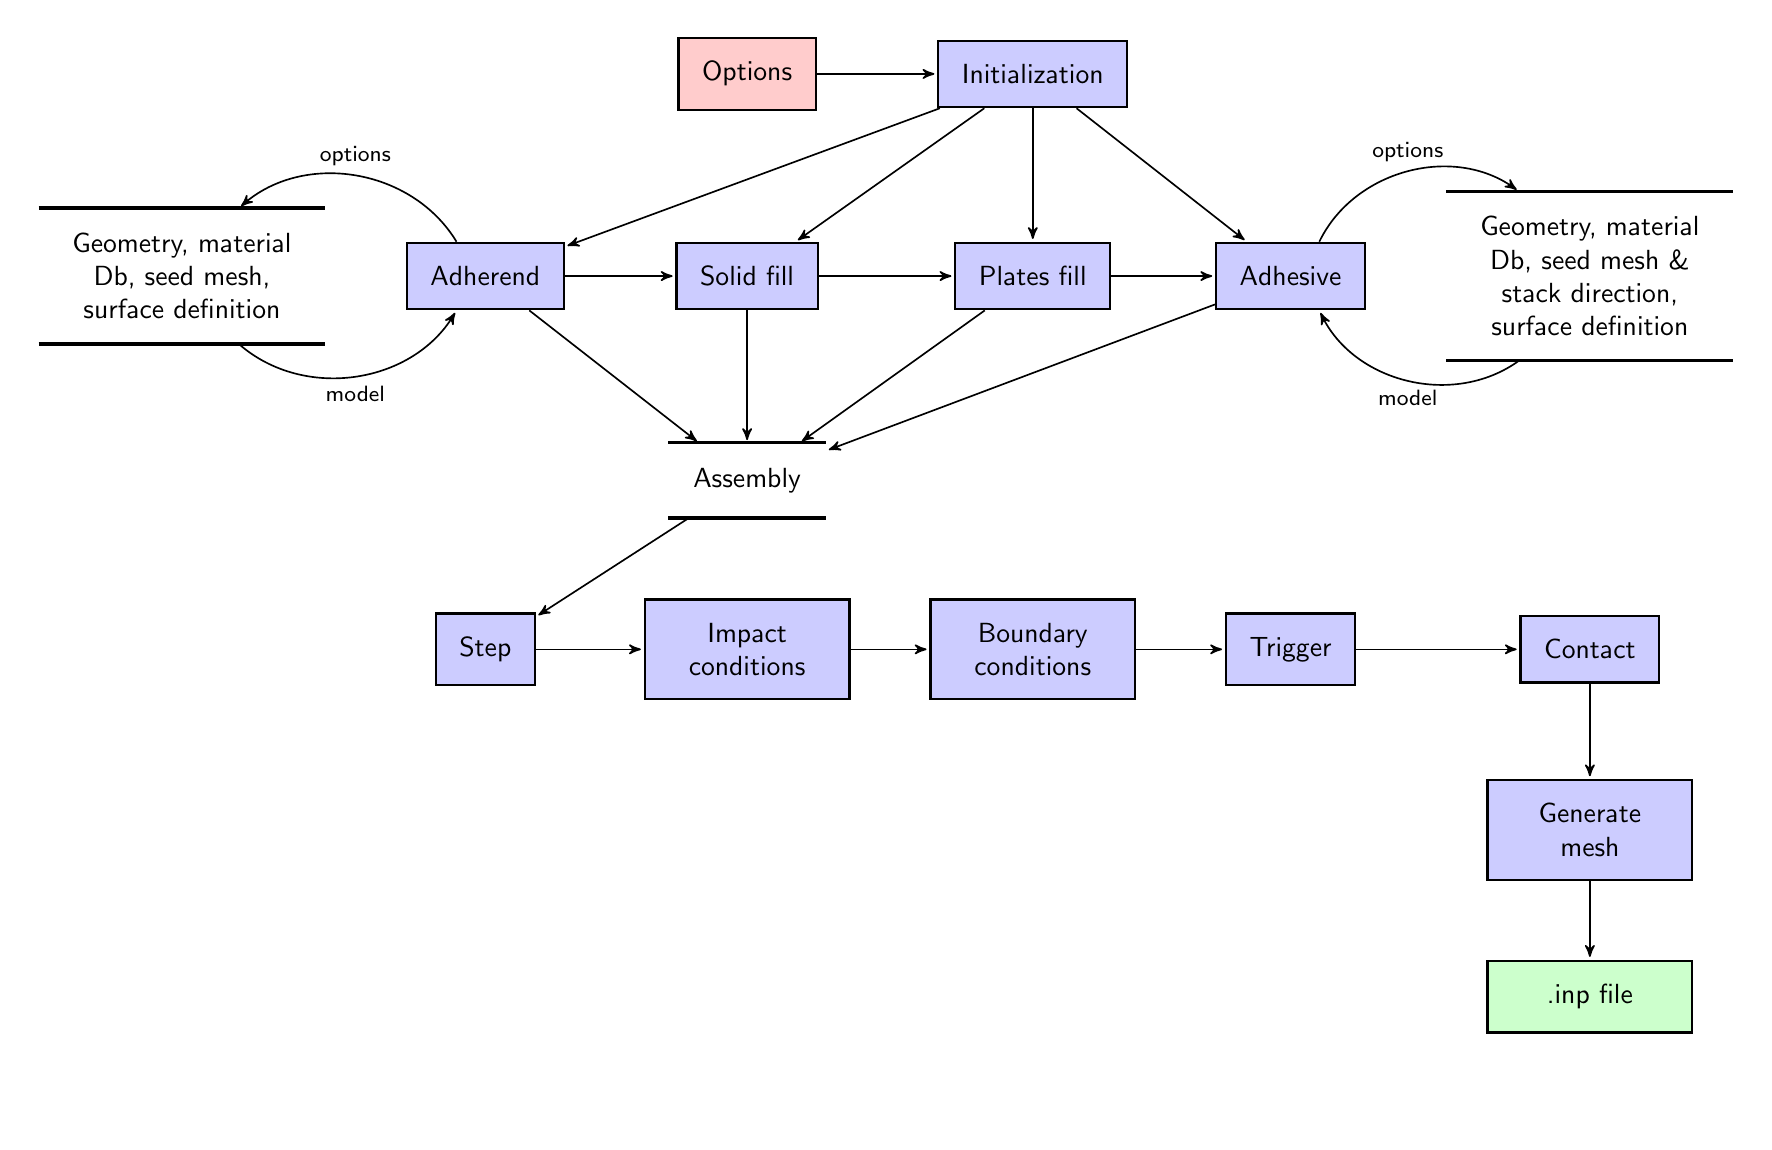
\begin{tikzpicture}[
  font=\sffamily,
  every matrix/.style={column sep=1cm,row sep=1cm},
  source/.style={draw,thick,fill=red!20,inner sep=.3cm},
  process/.style={draw,thick,fill=blue!20, inner sep=.3cm},
  sink/.style={source,fill=green!20},
  datastore/.style={draw,very thick,shape=datastore,inner sep=.3cm},
  dots/.style={gray,scale=2},
  to/.style={->,>=stealth',shorten >=1pt,semithick,font=\sffamily\footnotesize},
  every node/.style={align=center}]

  % Position the nodes using a matrix layout
  \matrix{
  	&& \node[source] (opc) {Options}; & \node[process] (init) {Initialization}; & \\
    
    \node[datastore](chapDB)[text width=3cm]{Geometry, material Db, seed mesh, surface definition}; & \node[process](chap){Adherend}; & \node[process](FSolid){Solid fill}; & \node[process](FPlat){Plates fill}; & \node[process](ads){Adhesive}; & \node[datastore](adsDB)[text width=3cm]{Geometry, material Db, seed mesh \& stack direction, surface definition};\\
    
    && \node[datastore](assembly){Assembly}; &&\\
    
    & \node[process](step){Step}; & \node[process](impact)[text width=2cm]{Impact conditions}; & \node[process](BC)[text width=2cm]{Boundary conditions}; & \node[process](trig){Trigger}; & \node[process](contct){Contact}; \\
    
    &&&&& \node[process](mesh)[text width=2cm]{Generate mesh}; \\
    &&&&& \node[sink](inp)[text width=2cm]{.inp file}; \\
    
    
      & & \\
  };

  % Draw the arrows between the nodes and label them.
   \draw[to] (opc) -- (init); 
   \draw[to] (init) -- (chap); 
   \draw[to] (init) -- (FSolid); 
   \draw[to] (init) -- (FPlat); 
   \draw[to] (init) -- (ads); 
   \draw[to] (chap) -- (assembly); 
   \draw[to] (FSolid) -- (assembly); 
   \draw[to] (FPlat) -- (assembly); 
   \draw[to] (ads) -- (assembly); 
   \draw[to] (chap) -- (FSolid); 
   \draw[to] (FSolid) -- (FPlat); 
   \draw[to] (FPlat) -- (ads); 
   \draw[to] (assembly) -- (step); 
   \draw[to] (step) -- (impact); 
   \draw[to] (impact) -- (BC); 
   \draw[to] (BC) -- (trig); 
   \draw[to] (trig) -- (contct); 
   \draw[to] (contct) -- (mesh); 
   \draw[to] (mesh) -- (inp);
   
   \draw[to] (chap) to[bend right=50] node[midway,above] {options} (chapDB);
   \draw[to] (chapDB) to[bend right=50] node[midway,below] {model} (chap);
   \draw[to] (ads) to[bend right=-50] node[midway,above] {options} (adsDB);
   \draw[to] (adsDB) to[bend right=-50] node[midway,below] {model} (ads);
     
 
\end{tikzpicture}
\end{document}